\documentclass[12pt]{book}
\usepackage{fontspec}
\usepackage{amsmath}
\usepackage{amsthm}
\usepackage{amssymb}
\usepackage[spanish]{babel}
\usepackage{authblk}
\usepackage{fullpage}
\usepackage[hyphens]{url}
\usepackage{hyperref}
\usepackage{graphicx}
\usepackage{xcolor}
\usepackage{minted}
\usepackage{parskip}
\usepackage[stable]{footmisc}
\usepackage{import}
\usepackage{exercise}
\usepackage{array}
\usepackage{csquotes}
\usepackage[style=reading, backend=biber, refsection=chapter, citereset=chapter]{biblatex}


\newtheorem{theorem}{Theorem}
\newtheorem*{note}{Nota}
\newtheorem*{important}{Importante}
\theoremstyle{definition}
\newtheorem{definition}{Definition}[chapter]
\newtheorem{exercise}[definition]{Ejercicio}
\definecolor{LightGray}{gray}{0.9}
\definecolor{Transparent}{gray}{1.0}
\setminted{breaklines, autogobble, escapeinside=||, bgcolor=LightGray}
\setmintedinline{breaklines, escapeinside=||, bgcolor=Transparent}
\usemintedstyle{manni}

\hypersetup{
    colorlinks=true,
    linkcolor=blue,
    filecolor=magenta,      
    urlcolor=cyan,
}

\setmainfont{Minion Pro}
\setmonofont{Source Code Pro for Powerline}[Scale=MatchLowercase]

\addbibresource{References.bib}

\graphicspath{{img/}}

\title{CC3002 - Metodologías de diseño y programación}

\author{Juan-Pablo Silva}
\author{Ignacio Slater}
\author{Beatriz Graboloza}
\affil{Departamento de Ciencias de la Computación, Universidad de Chile}

\date{\today}

\begin{document}
  \frontmatter
  \maketitle
  \tableofcontents
  % !TEX root = C:\Users\Ignacio\Documents\Escuela\CC3002 - Metodologías de Diseño y Programación\apunte-y-ejercicios\src\latex\Apunte.tex
\chapter{¿Por qué mi programa no funciona >.<?}

  Este capítulo es el comienzo de la parte central del apunte, a partir de aquí ya no nos va a 
  importar tanto \textit{Java} como lenguaje de programación, sino que lo veremos más como una 
  herramienta para ejemplificar los conceptos.
  El enfoque de éste y los capítulos que vienen será sobre \textbf{cómo diseñar} programas para
  solucionar problemas, dando énfasis a la calidad del código y a aprovechar de mejor forma la 
  programación orientada a objetos.

  \subimport{./}{Testing.tex}
  \subimport{./}{JUnit.tex}
  
  \nocite{*}
  \printbibliography[keyword=tdd]

  \mainmatter
  %% region : Parte 1
  \part{Herramientas necesarias y recomendadas}
    \import{./Herramientas/}{Java.tex}
    \import{./Herramientas/}{Git.tex}
    \import{./Herramientas/}{Cmder.tex}
  % endregion
  \part{Objetos en \textit{Java}}
    \chapter{Programación orientada a objetos}
  Hasta el momento, gran parte de lo que ustedes conocen es cómo escribir algoritmos 
  en los que realizan acciones siguiendo una lógica.
  La programación orientada a objetos (OOP) es un \textbf{paradigma} de computación 
  que se organiza en base a \textbf{objetos} en vez de acciones y \textbf{datos} en 
  lugar de lógica.

  Esto requiere un gran cambio de enfoque respecto a la programación imperativa 
  tradicional que están acostumbrados a usar puesto que el enfoque estará en cuáles 
  son los objetos que vamos a manipular en vez de la lógica para manipularlos.

  \section{Objetos}
    En el contexto de programación, un objeto es un elemento que tiene un 
    comportamiento y un estado definido, comúnmente llamados métodos y campos (este 
    último también aparece en la literatura como propiedades o variables de 
    instancia).
    
    El principal objetivo de utilizar objetos es poder crear estructuras para 
    almacenar información.

    Existen muchos beneficios de utilizar \textit{OOP}, pero algunas de las 
    propiedades más importantes son:

    \begin{itemize}
      \item \textbf{Transparencia:} La información almacenada dentro del objeto no 
        puede ser ``vista'' desde afuera de éste.
      \item \textbf{Encapsulación:} Cada objeto maneja sus propios datos y 
        funcionalidades.
      \item \textbf{Composición:} Todos los objetos pueden contener a otros (similar
        al concepto de composición de funciones en matemática: \(f \circ g\)).
      \item \textbf{Separación de responsabilidades:} Al utilizarse correctamente, 
        \textit{OOP} permite estructurar un programa en secciones, cada una 
        respondiendo a una responsabilidad específica, lo que añade modularidad al 
        código.
      \item \textbf{Polimorfismo:} Es la capacidad de un objeto de tipo \(A\) de verse
        y poder utilizarse como uno de tipo \(B\).
        Esto se verá en más detalle cuando se aplique \textit{OOP} en \textit{Java}
      \item \textbf{Delegación:} Cada objeto ejecuta solo las acciones que le 
        corresponden. 
        Si algo no le corresponde, entonces le manda un mensaje a otro (idealmente a 
        quien si le corresponde) que lo haga. 
        Básicamente es un "si no es mi trabajo que lo haga otro".
    \end{itemize}
    
    \subsection{Interacciones entre objetos}
      Por las propiedades de transparencia y encapsulación, un objeto no puede acceder 
      directamente a los componentes de otro, pero entonces: 
      ?`Cómo obtengo la información almacenada dentro de un objeto?
      
      Para interactuar con los objetos existe el concepto de \textit{mensaje}, este 
      concepto hace referencia a que en vez de acceder directamente a los componentes
      internos de un objeto, ``se le pide'' al objeto que realice una acción (esto se
      conoce como \textit{message passing}).
      Luego, cada objeto decide lo que debe hacer en base al mensaje que recibe.
      La manera en que un objeto decide qué acción tomar con cada mensaje se conoce 
      como \href{sec:method-lookup}{\textit{method-lookup}} y se explicará más 
      adelante.
    %
  %

  \section{Clases}
    Para introducir el concepto de clases empecemos con un ejemplo: si preparo dos 
    tortas siguiendo exactamente la misma receta, con los mismos ingredientes y la 
    misma preparación, entonces surge la duda, ?`son estas dos tortas la misma?
    La respuesta lógica es que no, son tortas individuales distintas entre ellas a 
    pesar de que su preparación haya sido la misma.
    
    Haciendo un símil con los objetos, podríamos decir que los ingredientes de la 
    torta son sus propiedades y la manera de prepararla son sus métodos, entonces 
    tendríamos dos objetos con las mismas propiedades y métodos pero distintos entre 
    sí, aquí es cuando entran las clases.
    Una clase es una manera de agrupar objetos, lo que informalmente podría llamarse 
    el \textit{tipo del objeto}.
    Más formalmente, una clase es una entidad en la programación orientada a objetos 
    a través de la cual se definen las características de todos los objetos 
    pertenecientes al grupo definido por la clase, por esta razón un objeto particular
    suele entenderse como una \textit{instancia de una clase}.

    Volviendo al ejemplo de las tortas, la clase podría verse como la receta utilizada
    para preparar los pasteles.

    La introducción del concepto de clases permite agregar otras características 
    fundamentales de \textit{OOP}.

    \subsection{Herencia}
      En programación la herencia se entiende como la \textit{especialización} de una 
      clase, esto se ilustra en la figura \ref{fig:canidae}\footnotemark

      \begin{figure}[ht!]
        \centering
        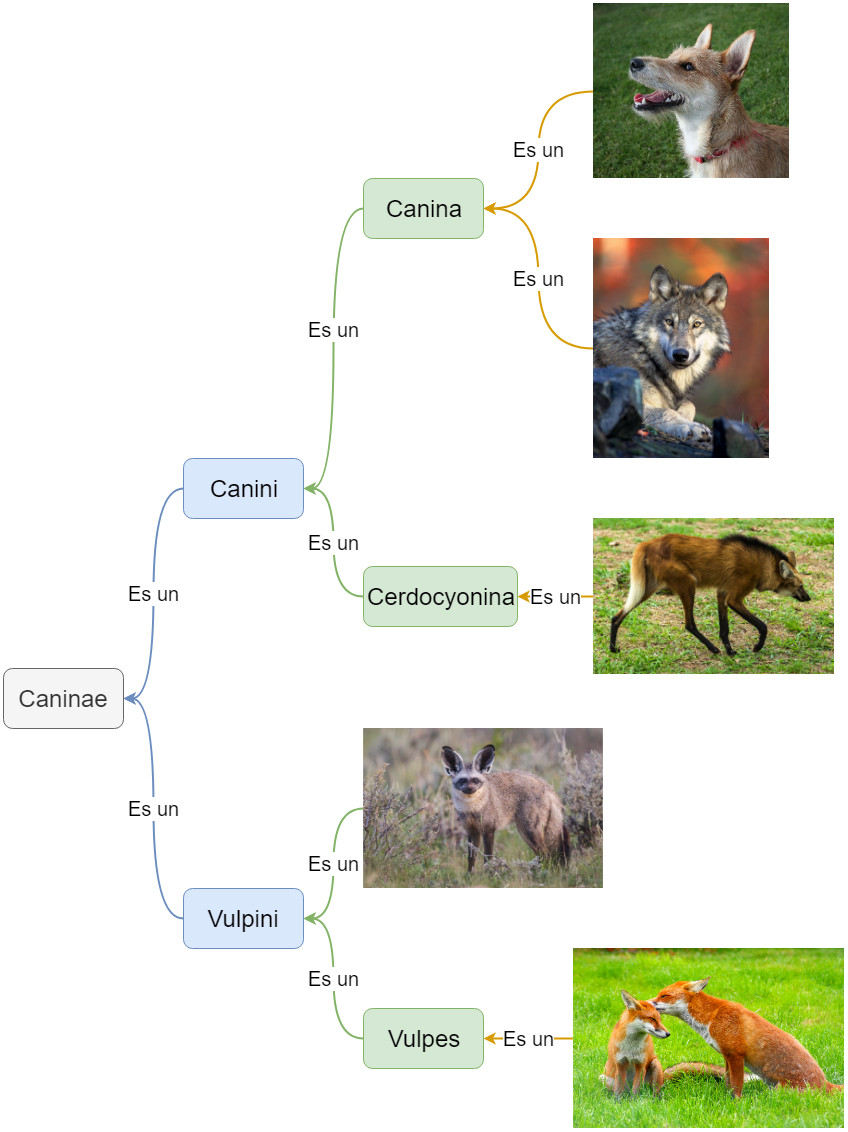
\includegraphics[width=0.8\textwidth]{Canidae.png}
        \caption{Ejemplo de herencia.}
        \label{fig:canidae}
      \end{figure}
      \footnotetext{Es importante resaltar que los animales no son objetos}

      En la figura se tiene que cada especie y subespecie es una clase, además se 
      puede apreciar que esto permite darle una organización jerárquica a nuestras 
      clases.
      Cuando hablamos de herencia en \textit{OOP}, se suele llamar a la clase que está
      heredando de otra como \textit{clase hija} o \textit{subclase} y a la otra como 
      \textit{clase padre} o \textit{superclase}.
      
      Esta propiedad es importante no sólo por la capacidad de definir subtipos, sino 
      que porque todas las clases hijas \textbf{heredan las funcionalidades} de la 
      clase padre.
      Como esto se cumple para todas las clases de la jerarquía, se tiene que la 
      herencia es una relación transitiva, de modo que \((\forall f,\, f \in 
      \mathcal{C}_0\ |\ \mathcal{C}_1 \subset \mathcal{C}_0 \wedge \mathcal{C}_2 \subset 
      \mathcal{C}_1 \implies f \in \mathcal{C}_2)\) 

      Como veremos más adelante, uno de los principales beneficios al momento de 
      utilizar herencia dentro del contexto de programación es evitar la duplicación 
      de código, pero es importante notar que esto es una consecuencia y no el 
      objetivo de utilizar herencia.
      En un programa bien construido la herencia \textbf{debe tener coherencia 
      lógica}, i.e. si bien tanto un avión como un pato pueden volar no tiene sentido
      crear una superclase para ambos porque son conceptualmente demasiado distintos 
      entre sí.
    %

    \subsection{Principios SOLID}
      Los \textbf{principios SOLID} son convenciones que se tienen en cuenta al momento de
      utilizar orientación a objetos y que permiten mantener una estructura robusta.
      Veremos más adelante que existen casos en los que se deben romper algunos de estos
      principios al momento de diseñar un programa para asegurar la mantenibilidad y 
      extensibilidad del código, pero dentro de lo posible siempre se debe intentar 
      respetar estos principios.

      \subsubsection{Single-responsibility principle}
        \textit{Una clase debe tener una y solamente una razón para cambiar, por lo que 
        toda clase debe tener una sola responsabilidad.}

        Para entender esto, considere el siguiente problema: tenemos figuras geométricas y 
        queremos calcular sus áreas.
        
        Una posible solución sería crear una clase que represente una figura geométrica y
        que de acuerdo al tipo de figura que nos interese, entonces podríamos tener un 
        método: \\
        \texttt{calculateArea(String)} que se utilice como 
        \texttt{calculateArea(``Rectangle'')}.
        Esto funcionaría, pero no respeta el principio, ya que tenemos una sola clase que
        se encarga de calcular el área de todas las figuras.

        Una solución que sí respeta el principio es la de crear clases distintas para cada 
        tipo de figura y que cada una de estas sepa cómo calcular su propia área (en esto 
        se puede aprovechar la herencia).
      %

      \subsubsection{Open-Closed principle}
        \textit{Los objetos o entidades deben estar abiertos para extenderse, pero 
        cerrados para modificarse.}

        Este principio hace referencia a que debe ser fácil agregar funcionalidades nuevas
        o específicas a un programa sin necesidad de cambiar las funcionalidades y 
        propiedades que ya tiene.
        Uno de los aprendizajes importantes del curso es cómo lograr cumplir con este 
        principio, los capítulos referentes a patrones y metodologías de diseño muestran 
        técnicas y patrones relevantes en este aspecto.

        El mismo ejemplo utilizado para el principio anterior aplica aquí.
        Si tenemos una sola clase que calcula las áreas de todo tipo de figuras, agregar 
        un nuevo tipo de figura implicaría modificar el método 
        \texttt{calculateArea(String)}, mientras que si se tiene cada figura como una 
        clase individual, agregar una nueva figura sería simplemente agregar una nueva 
        clase.
      %

      \subsubsection{Liskov's substitution principle}
        \textit{Sea \(q(x)\) una propiedad demostrable para objetos \(x\) de tipo \(T\). 
        Entonces \(q(y)\) debe ser demostrable para objetos \(y\) de tipo \(S\) donde \(S\)
        es un subtipo de \(T\).}\footnote{
          \url{https://en.wikipedia.org/wiki/Barbara_Liskov}
        }

        En terminos más simples, esto quiere decir que las subclases siempre deben ser 
        reemplazables por su clase padre.

        Consideren el siguiente problema, queremos crear un modelo para representar aves,
        crearemos dos en particular: \textit{Palomas} y \textit{Colibríes}.
        Podemos agrupar estas aves en una clase \textit{Ave} y definir que todas las aves
        pueden volar.
        Hasta aquí todo bien.

        ?`Pero qué pasa si ahora quiero agregar \textit{Pingüinos}?
        Los pingüinos no pueden volar, pero definimos que todas las aves pueden volar. 
        Nuestra definición inicial rompería entonces el principio de \textit{Liskov}.

        Una solución a esto sería crear una nueva clase que represente a las aves 
        voladoras y que sea un subtipo de Ave, de esta forma, un pingüino sería un ave, 
        mientras que una paloma sería un ave voladora.
      %

      \subsubsection{Interface segregation principle}
        \textit{Un cliente nunca debiera estar forzado a implementar una interfaz que no 
        ocupe o depender de métodos que no ocupe.}

        Una interfaz es una ``promesa'' que hace el programador con un cliente (quien use 
        el código) en la que define cuáles son las acciones que puede realizar cualquier 
        clase que implemente dicha interfaz.
        Este concepto se entenderá mejor cuando veamos aplicaciones de esto.

        Tomemos como ejemplo el mismo de las aves del principio anterior.
        La solución original que se planteó de darle a todas las aves la habilidad de 
        volar no rompia solamente el principio de Liskov sino que este también.
        Si hubieramos simplemente definido el pingüino como una subclase de ave, habríamos
        estado forzados a que el pingüino tuviera la capacidad de volar (aún cuando 
        podríamos haber definido el método de tal forma que no hiciera nada).

        La solución es la misma de antes.
      %

      \subsubsection{Dependency inversion principle}
        \textit{Las entidades deben depender de abstracciones y no de implementaciones. 
        Los modulos de alto nivel no deben depender de modulos de bajo nivel, sino que 
        deben depender de abstracciones.}

        Este principio suena más complicado de lo que realmente es.
        Lo que quiere decir es que al tener dependencias entre clases, la clase que tiene
        dependencia en otra no debe depender de implementaciones particulares de esta 
        clase, sino que de una abstracción de estas implementaciones.

        Usando las aves como ejemplo nuevamente, si tuvieramos una clase con un método 
        \texttt{alimentar} para alimentarlas, la implementación de esta clase no debe 
        depender de las implementaciones particulares, e.g. definir un método 
        \texttt{alimentar(Paloma)} estaría violando este principio.

        La manera correcta de implementar esto sin romper el principio sería crear un 
        único método \texttt{alimentar(Ave)}
      %
    %
  %
%
    \import{./}{De Python a Java.tex}
    \import{./}{java_1.tex}
    \import{./}{java2.tex}
  %
  \part{Patrones y metodologías de diseño}
    \chapter{\textit{Test Driven Development}}
      \label{ch:tdd}
    %
    \import{./}{gui.tex}
  %
  % \nocite{*}
  % \printbibliography
\end{document}